\documentclass[conference]{IEEEtran}
\IEEEoverridecommandlockouts

\usepackage{cite}
\usepackage{amsmath,amssymb,amsfonts}
\usepackage{algorithmic}
\usepackage{graphicx}
\usepackage{textcomp}
\usepackage{xcolor}
\usepackage[colorlinks=true, linkcolor=blue, citecolor=blue, urlcolor=blue]{hyperref}
\usepackage{cleveref}
\usepackage{pdflscape}
\usepackage{array}

\def\BibTeX{{\rm B\kern-.05em{\sc i\kern-.025em b}\kern-.08em
    T\kern-.1667em\lower.7ex\hbox{E}\kern-.125emX}}

\begin{document}
\bibliographystyle{IEEEtran}

\title{Autonomous and Manual Control of a Simulated Vehicle Using PID-Based Navigation in CoppeliaSim}

\author{
\IEEEauthorblockN{1\textsuperscript{st} Filipe Cavalheiro}
\IEEEauthorblockA{
\textit{DEEC} \\
\textit{NOVA FCT} \\
Lisbon, Portugal \\
https://orcid.org/0009-0000-1238-3975}
}

\maketitle

\begin{abstract}
This paper presents the development of a small autonomous ground vehicle in CoppeliaSim \cite{coppeliaSim}. The robot is capable of following predefined paths, avoiding obstacles, performing a parallel parking maneuver, and being manually driven by an operator using a commercial steering wheel controller. Navigation is implemented through a proportional-integral-derivative (PID) control system that regulates the steering angle based on heading errors. Experimental simulations demonstrate the effectiveness of the proposed approach and highlight the simplicity and robustness of PID-based navigation for small mobile robots.
\end{abstract}

\begin{IEEEkeywords}
mobile robots, PID control, path tracking, autonomous navigation, obstacle avoidance, CoppeliaSim, vehicle simulation
\end{IEEEkeywords}

\section{Introduction}
Autonomous vehicles and mobile robot navigation have been widely researched for decades, with numerous approaches relying on different sensors and control techniques. Despite the rise of advanced systems such as SLAM and deep-learning-based perception, PID control remains one of the most common solutions due to its simplicity, reliability, and ease of implementation.

This paper proposes a minimalistic autonomous navigation system that uses:  
(1) a single front-facing distance sensor,  
(2) a waypoint-based navigation controller, and  
(3) a PID regulator for steering control.

The robot is also equipped with a manual driving mode through a commercial Logitech MOMO steering wheel, enabling testing and comparison between manual and autonomous operation. The remaining sections are organized as follows: Section II introduces the simulation environment and system components, Section III describes the PID control strategy, Section IV presents the manual driving interface, Section V details the autonomous navigation and obstacle avoidance system, and Section VI explains the parallel parking procedure.

\section{System Components}
\subsection{CoppeliaSim}
CoppeliaSim provides a flexible and modular simulation environment for testing mobile robots and their control systems. The environment developed for this work includes straight paths, curves, and an obstacle course designed to evaluate both manual and autonomous navigation.

\begin{figure}[t]
    \centering
    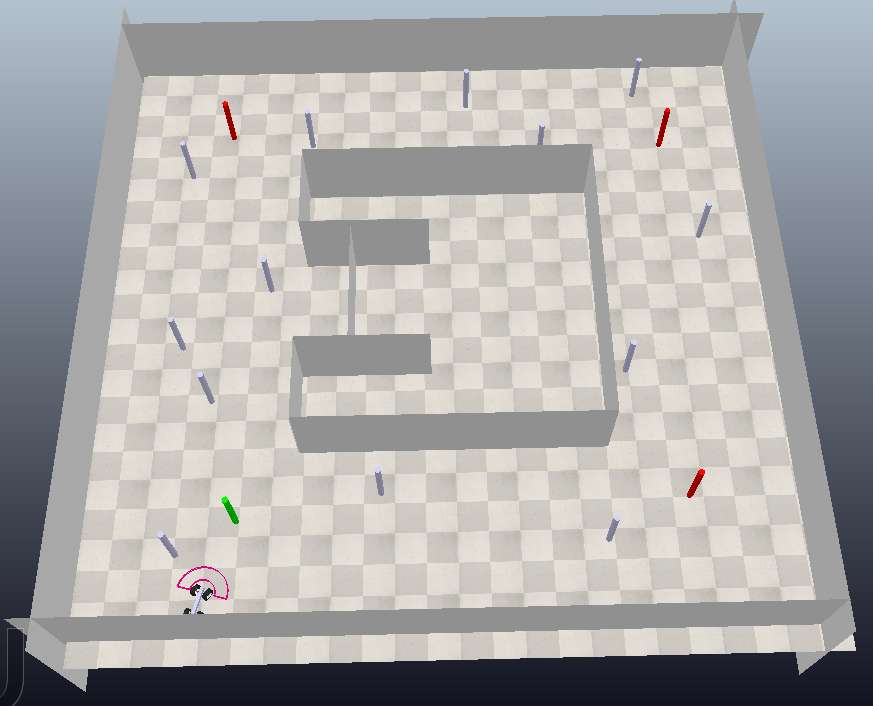
\includegraphics[width=8cm]{Images/obstacles_course.png}
    \caption{Obstacle course developed in CoppeliaSim.}
    \label{fig:obstacles_course}
\end{figure}

\subsection{PID controller}
\label{sec:PID}

The steering angle is controlled using a PID regulator that minimizes the heading error:
\begin{equation}
    u(t) = K_p e(t) + K_i \int_0^t e(\tau)\,d\tau + K_d \frac{d e(t)}{dt}
\end{equation}
where \(e(t)\) is the difference between the current orientation of the vehicle and the desired direction defined by the next waypoint. 
The current desired waypoint can be seen in green in \Cref{fig:obstacles_course}, as well as all other waypoints shown in red.

\subsection{Proposed vehicle}

\begin{figure}[t]
    \centering
    % Product photo not redistributed in this repository; it is in report.pdf.
    \IfFileExists{Images/momo_steering_wheel.jpg}{\includegraphics[width=8cm]{Images/momo_steering_wheel.jpg}}{\fbox{Logitech MOMO photo: see report.pdf}}
    \caption{Logitech MOMO steering wheel used for manual control.}
    \label{fig:momo}
\end{figure}

The developed vehicle, shown in (\Cref{fig:car}), uses rear-wheel traction, while the front axle is free to rotate and provides steering. Buttons on the wheel allow switching between three modes of navigation: Manual, Autonomous and Parking. The front mounted sensor allows for the detection of obstacles in a $180\deg$ range unsuring a collision free navigate in most circunstances despite being turn off during manual operation.

\section{Manual Driving}
The vehicle can be manually driven using a Logitech MOMO steering wheel and pedal set (\Cref{fig:momo}). This interface provides realistic vehicle control and allows the operator to navigate the simulated environment. Steering wheel rotation is mapped to a front-wheel steering angle in the range of $\pm 22.5^\circ$, while the two pedals control the wheel rotational speed between $\pm 2,\text{rad/s}$. Each pedal is responsible for applying a directional driving force: pressing the right pedal moves the vehicle forward, while pressing the left pedal applies reverse traction. Braking is achieved by not pressing any pedal. If both pedals are pressed simultaneously with equal force, the applied torques cancel each other and the vehicle remains stationary. In case the steering wheel is not connected to the computer a simple keyboard based input is used being [A, D] used for steering, [U, I] for velocity ajustment and [M, N, P] for mode changing.

\begin{figure}[t]
    \centering
    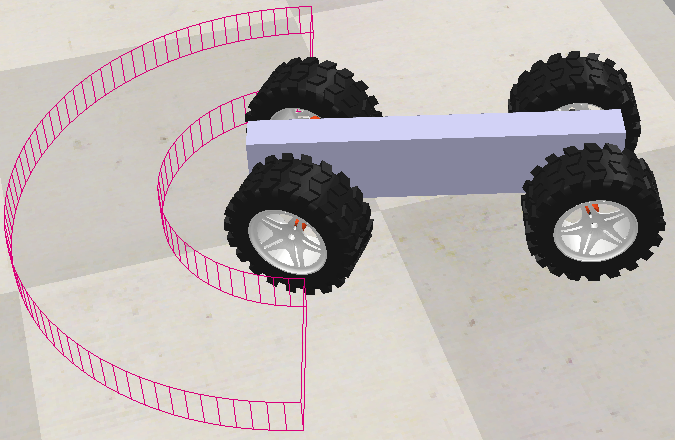
\includegraphics[width=8cm]{Images/car.png}
    \caption{Vehicle model used in the simulations.}
    \label{fig:car}
\end{figure}

\section{Navigation and Obstacle Avoidance}
\label{sec:Navigation_and_object_avoidance}

The robot follows a sequence of waypoints using the PID controller described in \Cref{sec:PID}. The heading error is computed as the angular difference between the current orientation and the direction of the vector connecting the robot to the next waypoint.

When the distance to the active waypoint becomes smaller than 0.2 m, the system automatically switches to the next waypoint.

Obstacle avoidance is handled by the front distance sensor. When an obstacle is detected, its angle relative to the vehicle's reference frame determines whether the robot should avoid it by steering left or right:
\begin{itemize}
    \item \textbf{Obstacle left} (\( \text{angle} < 90^\circ \)) → steer right
    \item \textbf{Obstacle right} (\( \text{angle} > 90^\circ \)) → steer left
\end{itemize}

This simple rule-based system proved effective for navigating around both static and dynamic obstacles. The speed during autonomous driving is fixed at a constant wheel rotation of $2 rad/s$.

\section{Parking}

\begin{figure}[t]
    \centering
    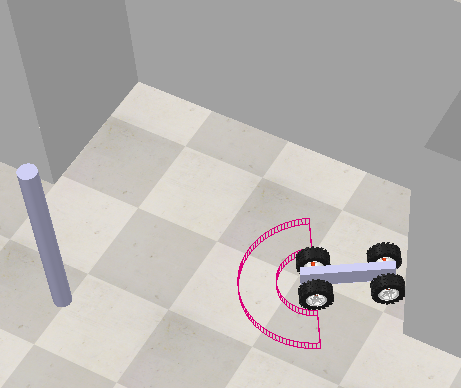
\includegraphics[width=8cm]{Images/parked_car.png}
    \caption{Vehicle parked using the autonomous parking routine.}
    \label{fig:parked_car}
\end{figure}

The parking mode uses the same PID steering controller but with reference points specifically placed to achieve a parallel parking maneuver. The volocity is also changed from the autonomous $2 rad/s$ to a more slow paced $1 rad/s$.

Once the vehicle detects that it has passed the available parking space, a waypoint is set at the front corner of the parking spot (aligned with the rear bumper of the vehicle ahead). The robot then moves forward until this waypoint is reached.  

A second waypoint is then placed behind the parking location (aligned with the front of the vehicle behind), causing the robot to reverse into the space. This ensures a smooth and collision-free parallel parking process. As shown in \Cref{fig:parked_car}, the vehicle successfully performs a parallel parking maneuver.

\section{TUI}
A quite simple text based user interface was also implemneted to help visualise the current system state, it is composed by the current oepration mode,  velocity as well as angle. it can be seen in \Cref{fig:TUI}.

\begin{figure}[t]
    \centering
    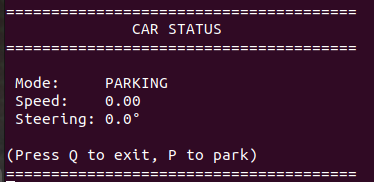
\includegraphics[width=8cm]{Images/TUI.png}
    \caption{Text User Interface (TUI).}
    \label{fig:TUI}
\end{figure}

\bibliography{references}
\end{document}
